% !TEX root =  ../main.tex 

\section{A framework for personalized biopsy schedules}
\label{sec : framework_pers_biop_sched}
The first step in creating a personalized schedule for biopsies is to come up with a model for Gleason scores, PSA levels and other patient specific characteristics. In PRIAS, PSA levels are measured at the time of induction, every 3 months for the first 2 years in the study and then every 6 months thereafter. Thus PSA levels can be modeled as a longitudinal outcome. As mentioned earlier, patients in PRIAS have a Gleason score of 6 or less at the time of induction in the study, and patients are removed from AS the first time GR takes place. Since our interest lies in finding the time of GR, we model it as a time to event outcome. While univariate modeling of the two aforementioned outcomes can be done separately using longitudinal model and survival models, but they are not independent. The association between the two exists because both are affected by the state of prostate cancer. To model the association between the two types of outcomes we use a joint model for time to event and longitudinal outcomes.

\subsection{Joint model for risk of GR and PSA levels}
\label{subsec : jm_definition}
Let $T_i^*$ denote the true GR time for the $i^{th}$ patient enrolled in an AS program. Let the vector of times at which a total of $g_i$ biopsies are conducted for the $i^{th}$ patient be denoted by $C_i = \{C_{i0}, C_{i1}, ... C_{ig_i}; C_{ij} < C_{ik}, \forall j<k \}$. $T_i^*$ cannot be observed directly and it is only known that it falls in an interval $(l_i, r_i]$, where $l_i = C_{i(g_i-1)}, r_i = C_{ig_i}$ if GR is observed, and $l_i = C_{ig_i}, r_i=\infty$ if patient drops out of AS. The latter is also known as right censoring. Let $\boldsymbol{y}_i$ denote the $n_i \times 1$ longitudinal outcome vector for the PSA levels of the $i^{th}$ patient. The population of interest is all the patients enrolled in AS. For a sample of $n$ patients from this population the complete data is denoted by $\mathcal{D}_n = \{T_i, l_i, r_i, \boldsymbol{y}_i; i = 1,...n\}$, where $T_i \epsilon (l_i, r_i]$ denotes the observed time of GR.\\

To model the evolution of the PSA measurements over time,  the joint model utilizes a linear mixed effects model. The longitudinal outcome $y_i(t)$ at a time $t$ is modeled as:

\begin{equation*}
\begin{split}
y_i(t) &= m_i(t) + \varepsilon_i(t), \\
&= \boldsymbol{x}_i^T(t) \boldsymbol{\beta} + \boldsymbol{z}_i^T(t) \boldsymbol{b}_i + \varepsilon_i(t)
\end{split}
\end{equation*}
%Do not introduce a space here, otherwise it starts a new paragraph
where, $m_i(t)$ denotes the true and unobserved value of the longitudinal outcome at time $t$. The measurement error $\varepsilon_i(t) \sim N(0, \sigma^2)$ is assumed normally distributed with variance $\sigma^2$. $\boldsymbol{\beta}$ denotes the vector of the unknown fixed-effects parameters. $\boldsymbol{b}_i \sim N(0, \boldsymbol{D})$ denotes the $q \times 1$ vector of random effects, assumed normally distributed with mean zero, and $q \times q$ covariance matrix $\boldsymbol{D}$. $\boldsymbol{b}_i$ and $\varepsilon_i(t)$ are assumed independent. $\boldsymbol{x}_i(t)$ and $\boldsymbol{z}_i(t)$ denote row vectors of the design matrices for the fixed and random effects, respectively. For non continuous longitudinal outcomes, joint models utilize Generalized linear mixed models \citep{rizopoulos2012joint}.\\

To model the effect of PSA measurements on risk of GR, joint models utilize a relative risk sub-model where the hazard of GR at any time point $t$, denoted by $h_i(t)$, depends on the history of true and unobserved values of PSA levels $\mathcal{M}_i(t) = \{m_i(v), 0\leq v \leq t\}$ measured up to that time point. Joint models offer flexibility in modeling this dependence. In its simplest form, the hazard may depend on instantaneous value of PSA $m_i(t)$ at time $t$. More sophisticated ones are dependence of hazard at time $t$ on PSA-DT, PSA velocity $m'_i(t) = \dfrac{d m_i(t)}{dt}$, or even on the cumulative effect of PSA $\int_0^t m_i(s) \,ds$ up to $t$. The fact that any functional form of dependence is possible, is evident from the following expression for hazard at time $t$:

\begin{equation*}
h_i(t \mid M_i(t), \boldsymbol{w}_i) = h_0(t) e^{\boldsymbol{\gamma}^T\boldsymbol{w}_i + f\{M_i(t), \boldsymbol{b}_i, \boldsymbol{\alpha}\}}
\end{equation*}
where $h_0(t)$ is the baseline hazard at time $t$. $\boldsymbol{w}_i$ is a vector of baseline covariates and $\boldsymbol{\gamma}$ are the corresponding parameters. The function $f(\cdot)$ parametrized by vector $\boldsymbol{\alpha}$ specifies the function form of longitudinal outcome that is used in the linear predictor of the relative risk model.\\

While $\boldsymbol{\alpha}$ controls the strength of association between the hazard of GR and features of the PSA history, the fact that both Gleason scores and PSA levels are internally related to a patient's health, is manifested by the random effects $\boldsymbol{b}_i$ in the model. The joint model postulates that given the random effects, time to GR and the different PSA measurements taken over time are all mutually independent. As mentioned earlier, in PRIAS study PSA-DT is used to decide the schedule of biopsies. Although PSA-DT is computed using observed PSA values, dependence on observed longitudinal history $\mathcal{Y}(t) = \{y_i(v), 0\leq v \leq t\}$ at any time $t$, is not the same as dependence on patient's health. On the contrary dependence on patient's health, manifested by $\boldsymbol{b}_i$ is same as dependence on future unobserved values of PSA. Thus the inference for the model parameters $\boldsymbol{\theta} = {\{\boldsymbol{\beta}^T, \boldsymbol{\gamma}^T, \boldsymbol{\alpha}^T, \sigma^2, \{d_{jk} \mid j=k=1,...q\}\}}^T$ doesn't change even if uncertainty in biopsy schedule $C_i$ is not modeled. The kernel of the corresponding joint likelihood conditional on the random effects and the model parameters is given by:

\begin{equation*}
p(T_i, l_i, r_i, \boldsymbol{y}_i \mid \boldsymbol{b}_i, \boldsymbol{\theta}) \propto p(T_i \mid l_i, r_i, \boldsymbol{b}_i, \boldsymbol{\theta}) p(\boldsymbol{y}_i \mid \boldsymbol{b}_i, \boldsymbol{\theta})
\end{equation*}

\subsection{Personalized scheduling approaches}
\label{subsec : pers_sched_approaches}
Once a joint model for GR and PSA levels is obtained, the next step is to use it to create personalized schedules for biopsies. In this section we present the various personalized biopsy scheduling approaches and their motivation. The personalized schedules that we propose are dynamic in nature and thus at any given time, only 1 future biopsy is scheduled. The age of the patient and entire PSA, repeat biopsy history up to that time point is considered while computing the time of next biopsy. To elucidate the scheduling methods, let us assume that the a personalized schedule is to be created a new patient enumerated $j$, who is not present in the original sample of patients $\mathcal{D}_n$. Further let us assume that this patient did not have a GR at their last biopsy performed at time $t$, and that the PSA measurements are available up to a time point $s$. Combining these two pieces of information, the predictive distribution $g(T^*_j)$ for time to GR for this patient is given by (conditioning on baseline covariates $\boldsymbol{w}_i$ is dropped for notational simplicity here onwards):

\begin{equation}
\label{eq : dyn_dist_fail_time}
\begin{split}
g(T^*_j) &= p(T^*_j \mid T^*_j > t, \mathcal{Y}_j(s), \mathcal{D}_n)\\
&= \int p(T^*_j \mid T^*_j > t, \mathcal{Y}_j(s), \boldsymbol{\theta}) p(\boldsymbol{\theta} \mid \mathcal{D}_n) \,d\boldsymbol{\theta}\\
&= \int \int p(T^*_j \mid T^*_j > t, \mathcal{Y}_j(s), \boldsymbol{b_j}, \boldsymbol{\theta}) p(\boldsymbol{b}_j \mid T^*_j>t, \mathcal{Y}_j(s), \boldsymbol{\theta})p(\boldsymbol{\theta} \mid \mathcal{D}_n) \,d\boldsymbol{b}_j \,d\boldsymbol{\theta}
\end{split}
\end{equation}
where $\mathcal{Y}_j(s)$ denotes the history of PSA measurements done up to time $s$. It can be seen that the predictive distribution depends on the observed longitudinal history via the random effects $\boldsymbol{b_j}$. The posterior distribution of the parameters $\boldsymbol{\theta}$ is obtained from the joint model fitted to the original data set of patients $\mathcal{D}_n$.\\

Given the predictive distribution $g(T^*_j)$, our goal is find the optimal time $u \geq \text{max}(t,s)$ of the next biopsy. To this end, we use principles from statistical decision theory in a Bayesian setting \citep{bergerDecisionTheory,robertBayesianChoice}. More specifically, we propose to choose future biopsy time $u$ by minimizing the posterior expected loss $E_g[L(T^*_j, u)]$, where the expectation is taken w.r.t. the predictive distribution $g(T^*_j)$. 

\begin{equation*}
E_g[L(T^*_j, u)] = \int_t^\infty L(T^*_j, u) p(T^*_j \mid T^*_j > t, \mathcal{Y}_j(s), \mathcal{D}_n) \,dT^*_j
\end{equation*}
Various loss functions $L(T^*_j, u)$ have been proposed in literature \citep{robertBayesianChoice}. The ones we utilize, and the corresponding motivations are presented next.

\subsubsection{Expected time of GR}
\label{subsubsec : exp_fail_time}
One of the reasons, patients did not comply with the existing PRIAS schedule was \textquoteleft complications on a previous biopsy \textquoteright. Therefore, it makes sense to have as less biopsies as possible. In the ideal case only 1 biopsy, performed at the exact time of GR is sufficient. Hence, neither a time which overshoots the true GR time $T^*_j$, nor a time which undershoots is preferred. In this regard, the squared loss function $L(T^*_j, u) = (T^*_j - u)^2$ and absolute loss function $L(T^*_j, u) = \mid T^*_j - u \mid$ have the properties that the posterior expected loss is symmetric on both sides of $T^*_j$. Secondly, both loss functions have well known solutions available. We first discuss the posterior expected loss for the squared loss function, given by:
%So the squared loss function satisfies our requirement of choosing a $u$ as close to the true GR time as possible. The is given by:
\begin{equation}
\label{eq : posterior_squared_loss}
\begin{split}
E_g[L(T^*_j, u)] &= E_g[(T^*_j - u)^2]\\
&=E_g[(T^*_j)^2] + u^2 -2uE_g[T^*_j]
\end{split}
\end{equation}
The posterior expected loss in equation \ref{eq : posterior_squared_loss} attains its minimum at $u = E_g[T^*_j]$, also known as expected time of GR.

\subsubsubsection{Estimation}
Since there is no closed form solution available for $E_g[T^*_j]$, for its estimation we introduce a construct called dynamic survival probability \citep{rizopoulos2011dynamic}. The dynamic survival probability $\pi_j(v \mid t, s)$ of patient $j$ is the survival probability at time $v$, conditional on the observed PSA history $\mathcal{Y}_j(s)$ and the fact that the patient did not have GR up to $t$. It is given by:

\begin{equation}
\pi_j(v \mid t, s) = Pr(T^*_j \geq v \mid  T^*_j >t, \mathcal{Y}_j(s), D_n), v \geq t
\end{equation}
The relationship between expected time of GR and dynamic survival probability is given by:

\begin{equation*}
E_g[T^*_j] = t + \int_t^\infty \pi_j(v \mid t, s) \,dv
\end{equation*}
Since the R package JMbayes already provides an implementation of $\pi_j(v \mid t, s)$, we preferred this approach over Monte Carlo methods to estimate $E_g[T^*_j]$ from the predictive distribution $g(T^*_j)$. There is no closed form solution available for the integral and hence we approximate it using Gauss-Kronrod quadrature. A limitation of \textquoteleft Expected time of GR though \textquoteright, is that it is practically useful only when the variance of predictive distribution $g(T^*_j)$ is small. The variance is given by:

\begin{equation}
\begin{split}
Var_g[T^*_j] &= E_g[{T^*_j}^2] - {E_g[T^*_j]}^2\\
&= 2 \int_t^\infty {(v-t) \pi_j(v \mid t, s) \,dv} - {\bigg(\int_t^\infty \pi_j(v \mid t, s) \,dv\bigg)}^2
\end{split}
\end{equation}
Once again, a closed form solution is not available for the variance expression. The variance however depends on both $t$ and $\mathcal{Y}_j(s)$. To elucidate the relationship between variance and observed information, we computed the variance at different time points for a couple of patients from the PRIAS study. The corresponding joint model fitted to the data set is discussed in section \ref{subsec : jm_fit_prias}. The first patient in question is patient nr. 405. He visited the hospital 53 times and was then right censored. 5 out those 53 visits were for biopsies. The variance of predictive distribution after each of those visits is shown in Figure \ref{fig : variance_pred_dist}. It is clear that the variance drops by a large margin each time a biopsy is conducted. i.e. when more information about $T^*_j$ is available. The effect of $\mathcal{Y}_j(s)$ on variance can be seen in Figure \ref{fig : variance_pred_dist_3174} which corresponds to patient nr. 3174, who visited the hospital 9 times and was censored after his last biopsy. The observed PSA measurements for this patient are shown in Figure \ref{fig : observed_psa_3174}. It can be seen that the variance doesn't depend on number of PSA measurements, but rather on the measurement values. For patient nr. 3174, variance drops quickly when PSA measurements increase sharply.  This becomes intuitive when we look at the model parameter estimates (section \ref{subsec : param_estimates_jm_fit_prias}), where rate of change of PSA $m'_i(t)$ is a strong predictor of the hazard of GR.

\begin{figure}[!htb]
    \centering
    \captionsetup{justification=centering}
    \begin{subfigure}[b]{0.45\textwidth}
        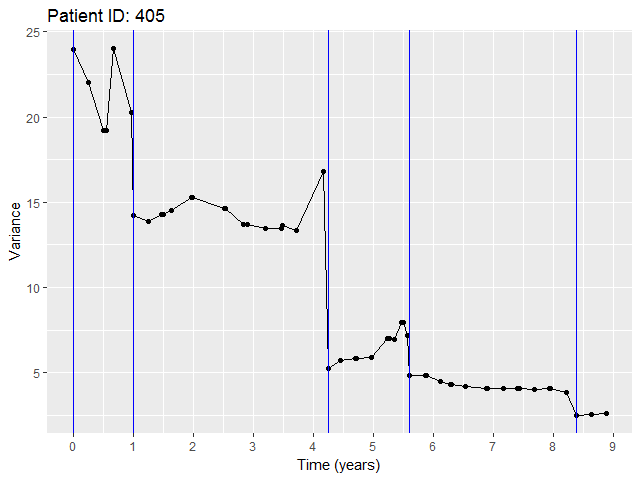
\includegraphics[width=\textwidth]{images/variance_pred_dist_405.png}
        \caption{Variance of the predictive distribution $g(T^*_j)$ over a period of 9 years for patient 405. Blue vertical lines indicate biopsies.}
        \label{fig : variance_pred_dist_405}
    \end{subfigure}   
    \begin{subfigure}[b]{0.45\textwidth}
        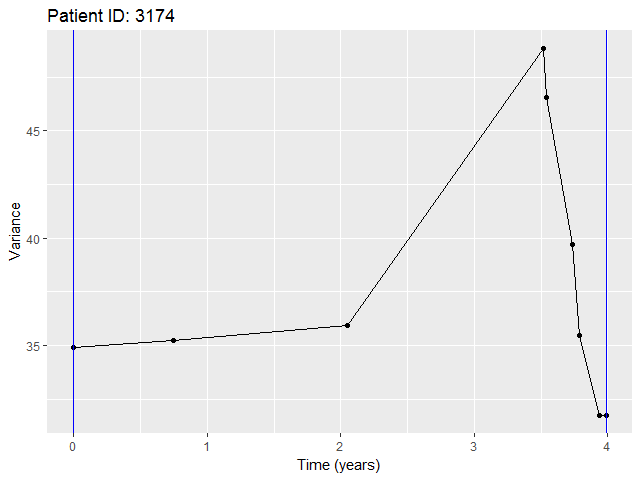
\includegraphics[width=\textwidth]{images/variance_pred_dist_3174.png}
        \caption{Variance of the predictive distribution $g(T^*_j)$ over a period of 4 years for patient 405. Blue vertical lines indicate biopsies.}
        \label{fig : variance_pred_dist_3174}
    \end{subfigure}
    \caption{Variance of the predictive distribution $g(T^*_j)$}\label{fig : variance_pred_dist}
\end{figure}

\begin{figure}[!htb]
    \centering
    \captionsetup{justification=centering}
    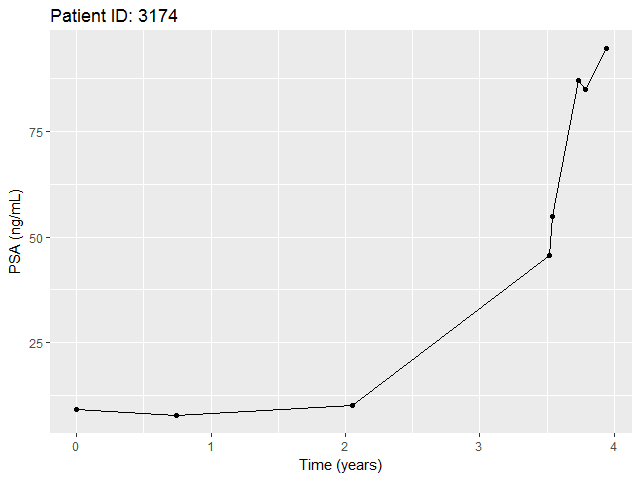
\includegraphics[width=0.5\textwidth]{images/observed_psa_3174.png}
    \caption{Observed evolution of PSA for patient 3174.}
    \label{fig : observed_psa_3174}
\end{figure}

\subsubsection{Dynamic risk of GR}
\label{subsubsec : dynamic_risk_definitions}
In a practical scenario it is possible that a doctor or a patient may not want to exceed a certain risk of GR $1 - \pi_j(u \mid t, s)$ since the last biopsy. This may be also useful in the cases where variance of $g(T^*_j)$ is high, rendering expected time of GR unsuitable. The personalized scheduling approach based on dynamic risk of GR, schedules the next biopsy at a time point $u$ such that the dynamic risk of GR is higher than a certain threshold $1-\kappa,\ \kappa \epsilon [0,1]$ beyond $u$. Or in other words the dynamic survival probability $\pi_j(u \mid t, s)$ is below a threshold $\kappa$ beyond $u$. In this regard, the posterior expected loss for the following multilinear loss function can be minimized to find the most optimal $u$:

\begin{equation}
\label{eq : loss_dynamic_risk}
L_{k_1, k_2}(T^*_j, u) =
    \begin{cases}
      k_2(T^*_j-u) & if(T^*_j > u)\\
      k_1(u-T^*_j) & \text{otherwise}
    \end{cases}       
\end{equation}
where $k_1 > 0$, $k_2 > 0$ are constants parameterizing the loss function. The posterior expected loss function $E_g[L_{k_1, k_2}(T^*_j, u)]$ obtains its minimum at $u = \pi_j^{-1}\Big\{\dfrac{k_1}{k_1 + k_2}\Big\}$ \citep{robertBayesianChoice}. The choice of $k_1, k_2$ is equivalent to the choice of $\kappa$. More specifically, $\kappa = \dfrac{k_1}{k_1 + k_2}$. When $k_1=k_2=1$, the multilinear loss function is equal to the absolute loss function $L(T^*_j, u) = \mid T^*_j - u \mid$. Since $\kappa = 0.5$ for absolute loss, time $u$ is the median of the predictive distribution $g(T^*_j)$.

\subsubsubsection{Choice of $\kappa$}
Since the value $\kappa$ dictates the biopsy schedule, its choice has important consequences. In certain cases it may be chosen on the basis of doctor's advice or the amount of risk that is acceptable to the patient. For e.g. if maximum acceptable risk is 75\% then $\kappa = 0.25$ and correspondingly, all $k_1, k_2 \mid k_1=\dfrac{k_2}{3}$ can be used in equation \ref{eq : loss_dynamic_risk} to calculate $u$. \\

While expert advice can be invaluable, it is also possible to automate the choice of $\kappa$. We propose to choose a $\kappa$ for which a binary classification accuracy measure \citep{lopez2014optimalcutpoints,sokolova2009systematic}, discriminating between cases and controls, is maximized. In PRIAS, cases are patients who experience GR and the rest are controls. However, a patient can be in control group at some time $t_a$ and in the cases at some future time point $t_b > t_a$, and thus time dependent binary classification is more relevant. In joint models, a patient $j$ is predicted to be a case if $\pi_j(t + \Delta t \mid t,s) \leq \kappa$ and a control if $\pi_j(t + \Delta t \mid t,s) > \kappa$ \citep{rizopoulosJMbayes}. The time window $\Delta t$ can be either chosen on a clinical basis (such as 1 year in PRIAS \textcolor{red}{\textbf{WHY 1 YEAR}}) or it can be chosen at a point where $AUC(t, \Delta t, s)$ \citep{rizopoulosJMbayes} is largest. i.e. $\Delta t$ for which the model has the most discriminative capability at time $t$. The binary classification accuracy measures we maximize to select the threshold $\kappa$ are the following (the binary classification measures are functions of $t, \Delta t, s$, although the notation is dropped for readability): 

\begin{itemize}
\item Accuracy: $ACC = \dfrac{TP + TN}{TP + FP + TN + FN}$, where TP, FP, TN and FN are the number of true positives, false positives, true negatives and false negatives at time point $t$. In this case if $k_1 = TP + TN$ and $k_2 = FP + FN$, then $\argmax{k_1, k_2} ACC$ gives the optimal $k_1, k_2$ or equivalently the $\kappa$.

\item Youden's index: $J = \text{Sensitivity} + \text{Specificity}- 1$,\\
where sensitivity is defined as $Pr(\pi_j(t + \Delta t \mid t,s) \leq \kappa \mid T^*_j \epsilon (t, t + \Delta t])$ and specificity is defined as $Pr(\pi_j(t + \Delta t \mid t,s) > \kappa \mid T^*_j > t + \Delta t)$. In this case if $k_1 = FP \cdot TP - FN \cdot TN$ and $k_2 = (TP+FN)(FP+TN) - k_1$, then $\argmax{k_1, k_2} J$ gives the optimal $k_1, k_2$ or equivalently the $\kappa$.

\item F1 Score: $F1 = \dfrac{2TP}{2TP + FP + FN}$. In this case if $k_1 = 2TP$ and $k_2 = FP + FN$, then $\argmax{k_1, k_2} F1$ gives the optimal $k_1, k_2$ or equivalently the $\kappa$.
\end{itemize}

\subsubsection{Mixed approach}

\subsubsection{Scheduling multiple biopsies}
\label{subsubsec : pers_sched_algorithm}
Scheduling biopsies using personalized schedules is an iterative process. Only one biopsy is scheduled at once, using all the information available up to that point in time. The information is manifested via the predictive distribution $g(T^*_j)$. It is important to note that new biopsy times are only proposed when the patient visits the hospital for a PSA measurement or for biopsy, since $g(T^*_j)$ is updated only at these time points. If a biopsy is conducted at time $t$, then scheduling the next biopsy at time $u \geq \text{max}(t,s)$ for patient $j$ is the goal. Although the predictive distribution $g(T^*_j)$ is updated with the new information $T^*_j > t$, there are a couple of restrictions on time $u$, namely:

\begin{enumerate}
\item Two consecutive biopsies should have a gap of at least 1 year between them. i.e. $u \geq t + 1$. Given the medical side effects of biopsies, the 1 year gap is strongly advised for patients enrolled in PRIAS. However, the personalized scheduling methods do not take this rule into account.
\item Although it is required that $u \geq \text{max}(t,s)$, the personalized scheduling methods may propose to perform a biopsy at a time $u \epsilon (t, s]$. The reason is that, GR is not a terminating event, and so the patients continue to visit for PSA measurements. The support of the predictive distribution $g(T^*_j)$, however does not depend on last time of PSA measurement $s$, and remains $(t, \infty)$.
\end{enumerate}
 
Lastly, it is extremely likely that on consecutive visits to the hospital for PSA measurements, the personalized biopsy time is postponed or preponed. The choice of time of biopsy from consecutive visits is not clear. To resolve these issues, we propose to supplement the personalized scheduling methods with the following algorithm.

\subsubsubsection{Algorithm}
Let us assume that patient $j$ had their latest biopsy at time $T^l_j$, and the latest available PSA measurement is from the current visit to the hospital, at time $T^{cv}_j$. The predictive distribution for time of GR is given by $p(T^*_j|T^*_j > T^l_j, \mathcal{Y}_j(T^{cv}_j), \mathcal{D}_n)$. Further let,

\begin{enumerate}
\item $T^p_j$ denote the time at which a biopsy is proposed by personalized scheduling methods.
\item Let $T^s_j$ denote the time at which a biopsy is scheduled. This is not necessarily equal to the proposed time $T^p_j$, but rather a time devoid of the problems mentioned earlier. This time is generated from the algorithm.
\item $T^{nv}_j$ denote the time of the next visit for PSA.
\item $N^b_j$ denote the counter for number of biopsies conducted up to time $T^l_j$, excluding the biopsy done at the time of induction in AS.
\end{enumerate}
Using these constructs, we have proposed an algorithm to schedule multiple biopsies. It is shown in Figure \ref{fig : sched_algorithm}. 

\begin{figure}[!htb]
\centering
\captionsetup{justification=centering}
\resizebox{0.65\columnwidth}{!}{%

\begin{tikzpicture}
\node (start) [startstop] {
Enter Active Surveillance.
\begin{enumerate}
\item Conduct a biopsy.
\item Set $t=T^{nv}=0$ 
\item Set $u = \infty$
\end{enumerate}
};

\node (takePSA) [process_wide_5cm, below=1cm of start] {
\begin{enumerate}
\item Measure PSA at $T^{nv}$ 
\item Set $s=T^{nv}$
\end{enumerate}
};

\node (propTime) [process_wide_3pt5cm, below=1cm of takePSA] {
\begin{enumerate}
\item Set $u^{pv} = u$ 
\item Update $g(T^*_j)$ 
\item Propose $u$
\end{enumerate}
};

\node (decision1) [decision, below = 1.5cm of propTime] {$u < u^{pv}$};
\node (pro6) [process, right = 1.35cm of decision1] {Set $u = u^{pv}$};

\node (decision5) [decision, left=1.5cm of decision1] {$u \leq s$};

\node (pro5) [process, below=1.5cm of decision5] {Set $u = s$};

\node (decision2) [decision, below=0.5cm of decision1] {$u - t > 1$};

\node (decision4) [decision, right=1.5cm of decision2] {$u > T^{nv}$};

\node (pro3) [process_wide_3pt5cm, below=1cm of decision2] {
\begin{enumerate}
\item Conduct Biopsy at $t + 1$ 
\item Set $t = t + 1$
\end{enumerate}
};

\node (pro4) [process_wide_3pt5cm, below=1cm of decision4] {
\begin{enumerate}
\item Conduct Biopsy at $u$
\item Set $t = u$
\end{enumerate}
};

\node (decision3) [decision, below=1cm of pro3] {$\mbox{Gleason} > 6$};
\node (pro7) [process, left=1cm of decision3] {Set $u=\infty$};

\node (stop) [startstop, below = 1cm of decision3] {Remove patient from AS};

\draw [arrow] (start) -- (takePSA);
\draw [arrow] (takePSA) -- (propTime);
\draw [arrow] (propTime) -- (decision1);
\draw [arrow] (decision1) -- node[anchor=south] {Yes} (decision5);
\draw [arrow] (decision5) -- node[anchor=east] {Yes} (pro5);
\draw [arrow] (pro5) -- (decision2);
\draw [arrow] (decision1) -- node[anchor=south] {No} (pro6);
\draw [arrow] (decision5) -- node[anchor=south] {No} (decision2);
\draw [arrow] (pro6) -- (decision4);
\draw [arrow] (decision4.east) |- ([xshift=0.35cm, yshift=-4.15cm]pro6.north east) |- node[anchor=south] {Yes} (takePSA);
\draw [arrow] (decision2) -- node[anchor=south] {Yes} (decision4);
\draw [arrow] (decision2) -- node[anchor=east] {No} (pro3);
\draw [arrow] (pro3) -- (decision3);
\draw [arrow] (pro4) |- (decision3);
\draw [arrow] (decision3) -- node[anchor=east] {Yes} (stop);
\draw [arrow] (decision4) -- node[anchor=east] {No} (pro4);
\draw [arrow] (decision3) -- node[anchor=south]{No} (pro7);
\draw [arrow] (pro7.west)|- ([xshift=-0.35cm, yshift=-7.8cm]pro5.north west) |- (propTime);
\end{tikzpicture}

}%


\caption{Algorithm for scheduling multiple biopsies using personalized schedules.} 
\label{fig : sched_algorithm}
\end{figure}